\chapter{Sensibilidad al umbral de 10 m}\label{A:Sensibilidad_10m_clasificacion}

\subsection*{Sensibilidad al umbral de reposo}

Para evaluar la elección del umbral de $10\,\mathrm{m}$, repetimos la clasificación de los días y la evaluación de todos los
modelos con umbrales de $11$ y $13\,\mathrm{m}$, manteniendo sus parámetros (Figura~\ref{fig:umbral}). En los datos, al subir
el umbral solo pasan días de exploración y retorno a reposo: la fracción de días de reposo pasa de $22.6\%$ a $25.6\%$ y
$31.0\%$, mientras que la de cambio de refugio se mantiene en torno al $44.5\%$.

Con $11\,\mathrm{m}$, la fracción de días del modelo de reposo (solo error del GPS) que se clasifican correctamente pasa del
$77\%$ al $83\%$, y el MSD diario de los días de reposo sigue siendo compatible con el de una tortuga quieta. Con
$13\,\mathrm{m}$, en cambio, el MSD diario de los días clasificados como reposo crece por encima del que produce el error del
GPS ($34$ contra $22\,\mathrm{m^2}$ a $240\,\mathrm{min}$): la categoría de reposo empieza a incluir excursiones reales.
Además, la mitad de los días del modelo de exploración y retorno pasa a clasificarse como reposo.

Un umbral de $11\,\mathrm{m}$ sería, por lo tanto, una alternativa razonable, que reduce la confusión entre el reposo y el
error del GPS sin mezclar excursiones reales en la categoría de reposo. Adoptarlo requeriría recalibrar el modelo de
exploración y retorno y el adelanto de la sigmoide de salida, ya que la salida detectada se retrasa al aumentar el umbral.
Mantenemos $10\,\mathrm{m}$ en el cuerpo de la tesis.

\begin{figure}[H]
    \centering
    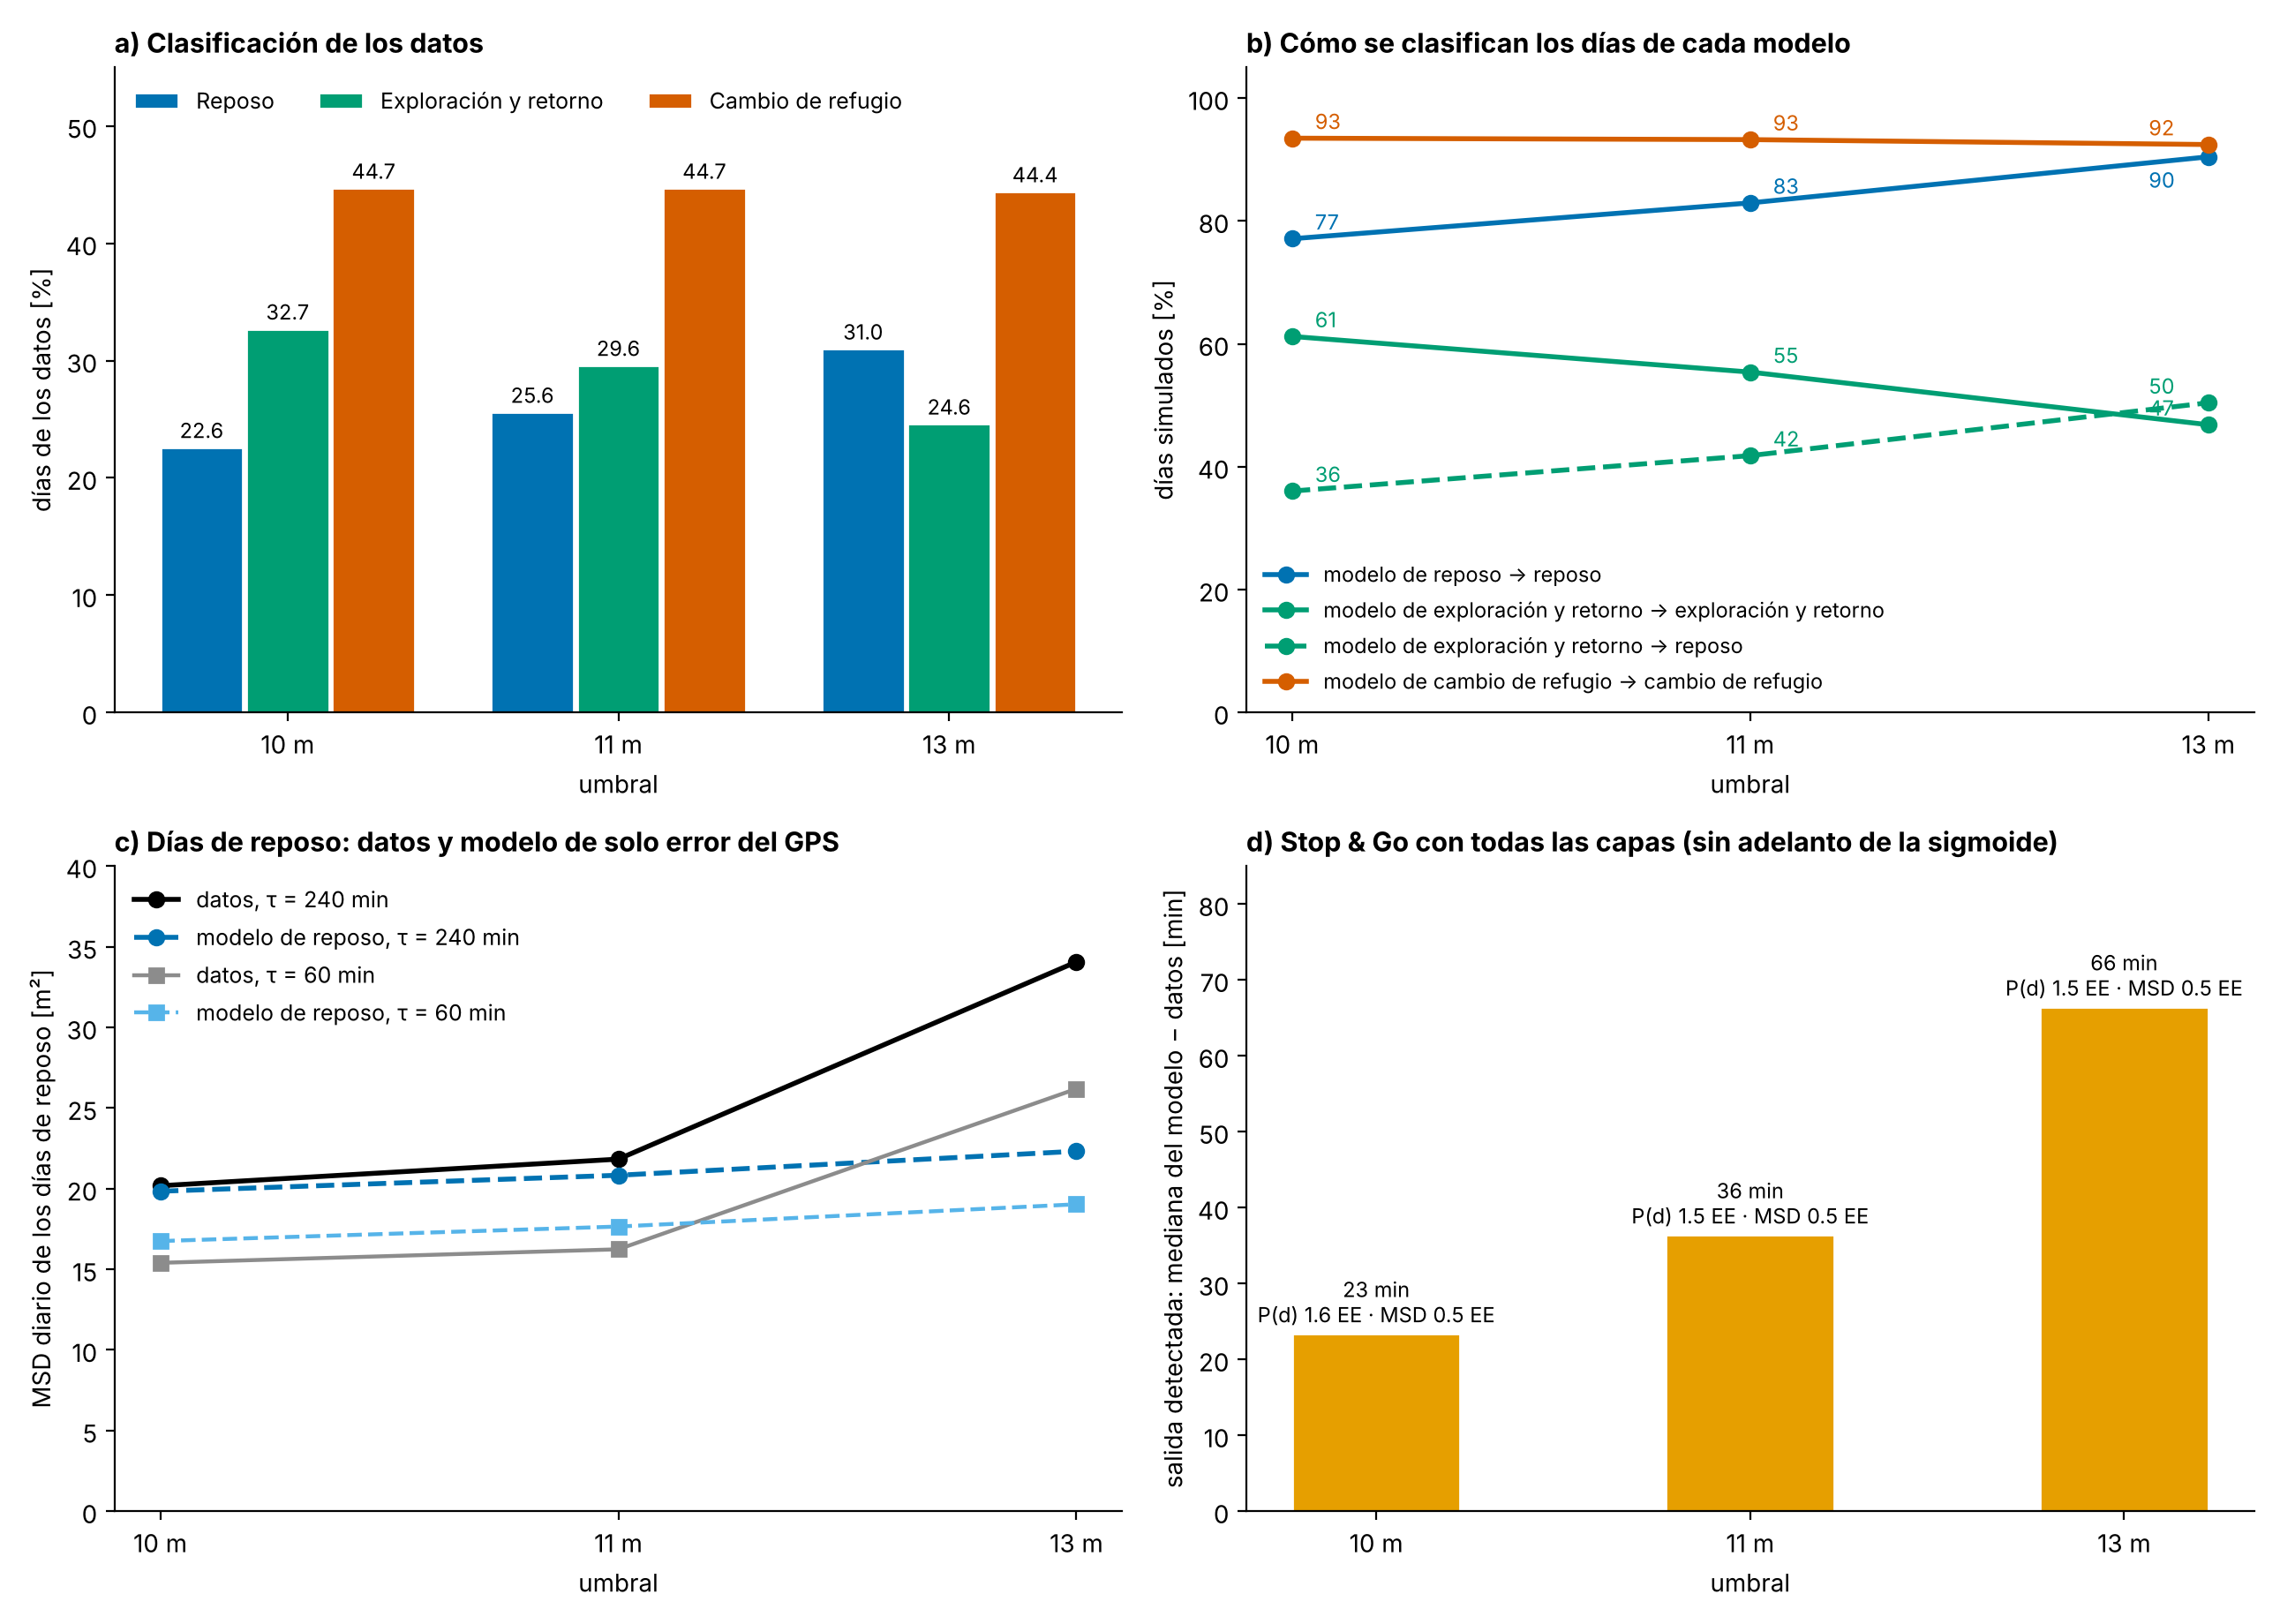
\includegraphics[width=\textwidth]{comparacion_umbral_10_11_13.png}
    \caption{Sensibilidad al umbral de reposo ($10$, $11$ y $13\,\mathrm{m}$). a) Clasificación de los días de los datos.
    b) Fracción de días simulados de cada modelo que se clasifica en cada tipo (promedio de las tres épocas).
    c) MSD diario de los días de reposo en los datos y en el modelo de solo error del GPS, a $60$ y $240\,\mathrm{min}$.
    d) Diferencia entre las medianas de la hora de salida detectada en el Stop \& Go y en los datos, con la distancia
    a los datos en el P(d) y en el MSD diario.}
    \label{fig:umbral}
\end{figure}

%%% Local Variables: 
%%% mode: latex
%%% TeX-master: "template"
%%% End: 
